\documentclass{article}[18pt]
\usepackage{../../../../../format}
\lhead{ADS - Andrei}
\lstset{language=Python,
	basicstyle=\ttfamily,
	keywordstyle=\bfseries,
	showstringspaces=false,
	morekeywords={if, else, then, print, end, for, do, while},
	tabsize=4,
	mathescape=true
}

\begin{document}
\begin{center}
\underline{\huge Trees}
\end{center}
\textbf{Tree} - A connected graph without cycles\\
\textbf{Parent} - The node above a node\\
\textbf{Child} - The node below a node\\
\textbf{Leaf} - Child-less nodes
\subsection{Using trees to store data}
In a binary tree, each node has:
\begin{itemize}
	\item Pointer to parent (or NIL, or to itself, if root)
	\item Pointer to left child (or NIL, or to itself, if there isn't one)
	\item Pointer to right child (or NIL, or to itself, if there isn't one)
	\item Payload
\end{itemize}
Binary trees are useful to store data, giving fast insert, lookup and delete operations.
\section{BST}
A binary search tree (BST) is a tree in which no node has more than two children\\
\\
You must build and maintain the tree such that it's true for every node v of the tree that
\begin{itemize}
	\item all elements in its left sub tree are "smaller" than v
	\item all elements in its right sub tree are "bigger" than v
\end{itemize}
Smaller and bigger refer to the payload. The left/right sub-tree refers to the tree rooted in a node's left/right child
\subsection{Traversals}
Starting with root:
\begin{itemize}
	\item In order: Recurse into left sub-tree, print payload, recurse into right sub-tree
	\item Pre-order: Print payload, recurse into subtrees
	\item Post-order: recurse into sub-trees, print payload
\end{itemize}
\subsection{Code for a BST}
Initialising a node:
\begin{lstlisting}
class Node:
	"""
	Tree node: left and right child + data which can be any object
	"""
	def __init__(self, data):
	"""
	Node constructor
	@param data node data object
	"""
	self.left = None
	self.right = None
	self.data = data
\end{lstlisting}
Inserting a node:
\begin{lstlisting}[tabsize=4]
class Node:
	...
	def insert(self, data):
		"""
		Insert new node with data
		@param data node data object to insert
		"""
		if data < self.data:
			if self.left is None:
				self.left = Node(data)
			else:
				self.left.insert(data)
		else:
			if self.right is None:
				self.right = Node(data)
			else:
				self.right.insert(data)
\end{lstlisting}
Looking up a value:
\begin{lstlisting}
class Node:
	...
	def lookup(self, data, parent=None):
	"""
	Lookup node containing data
	param data node data object to look up
	param parent node's parent
	returns node and node's parent if found or None, None
	"""
	if data < self.data:
		if self.left is None:
			return None, None
		return self.left.lookup(data, self)
	elif data > self.data:
		if self.right is None:
			return None, None
		return self.right.lookup(data, self)
	else:
		return self, parent
\end{lstlisting}
\subsubsection{Deleting}
Deleting is the most difficult operation on a BST.\\
\\
We first do a lookup on the element that we wish to remove. If that returns "not found" then we're done.\\
\\
Otherwise, three cases need to be considered:
\begin{itemize}
	\item If a node is a leaf then simply remove it
	\item If a node has one child then remove and replace it with that one child - list the sub tree up
	\item If a node has two children
\end{itemize}
Counting children:
\begin{lstlisting}
class Node:
	...
	def children_count(self):
		"""
		Returns the number of children
		@returns number of children: 0, 1, 2
		"""
		if node is None:
			return None
		cnt = 0
		if self.left:
			cnt += 1
		if self.right:
			cnt += 1
		return cnt
\end{lstlisting}
Deleting a node
\begin{lstlisting}
class Node:
	...
	def delete(self, data):
	"""
	Delete node containing data
	@param data node's content to delete
	"""
	# get node containing data
	node, parent = self.lookup(data)
	if node is not None:
		children_count = node.children_count()
	
	if children_count == 0:
		# if node has no children, just remove it
		if parent.left is node:
			parent.left = None
		else:
			parent.right = None
		del node
		
	elif children_count == 1:
		# if node has 1 child
		# replace node by its child
		if node.left:
			n = node.left
		else:
			n = node.right
		if parent:
			if parent.left is node:
				parent.left = n
			else:
				parent.right = n
		del node
		
	else:
		# if node has 2 children
		# find its successor
		parent = node
		successor = node.right
		while successor.left:
			parent = successor
			successor = successor.left
		# replace node data by its successor data
		node.data = successor.data
		# fix successor's parent's child
		if parent.left == successor:
			parent.left = successor.right
		else:
			parent.right = successor.right
\end{lstlisting}
\section{RedBlack trees}
BST property: for all nodes v with key k:
\begin{itemize}
	\item nodes in left subtree has keys $<k$
	\item nodes in right subtree have keys $>k$
\end{itemize}
Have seen simple BST operations:
\begin{itemize}
	\item Lookup
	\item Minimum, maximum
	\item Predecessor, successor
\end{itemize}
All take $\mathcal{O}(h)$ time, h height of tree\\
\\
This is OK if the BST is \textbf{balanced}, then $h=\mathcal{O}(\log n)$\\
\textbf{Bad} if the BST is \textbf{degenerated}, then $h=\Omega(n)$
\subsection{The idea}
A red black tree is an ordinary BST with one extra bit of storage per node, it's colour: red or black\\
\\
Constraining how nodes can be coloured results in (approximate) balancedness of tree\\
\\
Assumption: if either parent, left, or right does not exist, pointer to NULL\\
\\
Regard NULLs as leaves of tree, thus normal nodes are internal.\\
\\
A BST is a red-black tree if:
\begin{enumerate}
	\item Every node is either red or black
	\item the root is black
	\item every leaf (NULL) is black
	\item Red nodes have black children
	\item for all nodes, all paths from node to descendant leaves contain the same number of black nodes`
\end{enumerate}
\begin{center}
	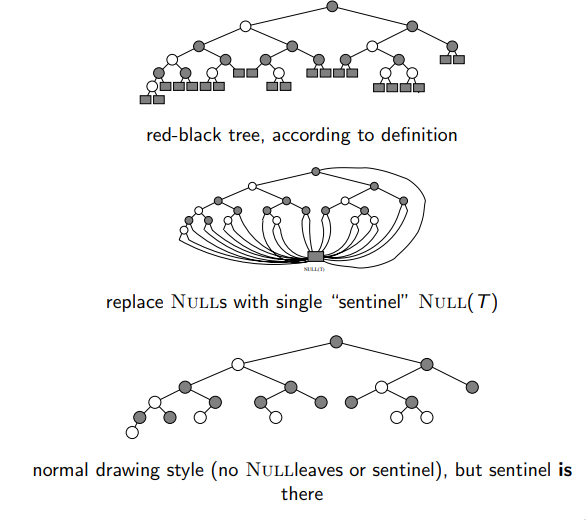
\includegraphics[scale=0.7]{redblack}
\end{center}
A redblack tree with n internal nodes has height at most $2\log(n+1)$\\
This means that all Lookup, min, max, successor, predecessor all have worst case $\mathcal{O}(\log n)$ time
\subsection{Rotations}
In order to maintain the red-black property, rotations must be used.\\
\\
There is the option of a left or right rotation, under the assumptions:
\begin{itemize}
	\item left rotation on x: right child not NULL
	\item right rotation on x: left child not NULL
\end{itemize}
\begin{center}
	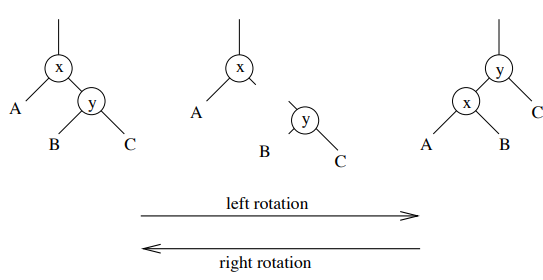
\includegraphics[scale=0.7]{rotate}
\end{center}
\begin{center}
	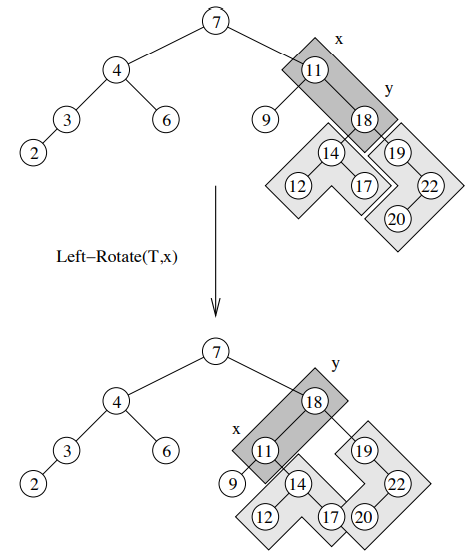
\includegraphics[scale=0.7]{rotate1}
\end{center}
This can be done in $\mathcal{O}(\log n)$ time\\
\\
Suppose we insert a new node z\\
\\
First, ordinary BST insertion of z according to key value (walk down from root, open new leaf)\\
\\
The, colour z red\\
\\
We may have violated the red-black property\\
\\
Then call the fixup procedure to restore the red black property
\section{Heaps}
Heaps are also trees, but typically assumed to be stored in a flat array
\begin{itemize}
	\item each tree node corresponds to an element of the array
	\item the tree is complete except perhaps the lowest level, filled left to right
	\item heap property: for all nodes v in the tree, \texttt{v.parent.data $>=$ v.data}
	\item This is a max heap (for min heaps, \texttt{v.parent.data $=<$ v.data})
\end{itemize}
Heap represented as an array A has two attributes:
\begin{itemize}
	\item Length(A) - The size of the array
	\item HeapSize(A) - The size of the heap stored within the array
\end{itemize}
Clearly, Length(A)$\geqslant$HeapSize(A) at all times
\subsection{Array indices}
Assume we start counting at position 1, then:
\begin{itemize}
	\item The root is in A[1]
	\item parent(i)=A[i/1] (integer division, rounds down)
	\item left(i)=A[2i]
	\item right(i)=A[2i+1]
\end{itemize}
\subsection{Why use heaps?}
Heaps are very good data structures for priority queues as sorting
\begin{lstlisting}
HeapExtractMax(A)
ret = A[1] // biggest element (highest priority)
A[1] = A[HeapSize(A)]
HeapSize(A) = HeapSize(A)-1
Heapify(A,1,HeapSize(A))
return ret
\end{lstlisting}
\subsection{Heapify}
Heapify changes a tree into a heap\\
\\
Idea:
\begin{itemize}
	\item Starting at the root, identify largest of current node v and its children
	\item Suppose largest element is in w
	\item If $w\neq v$
	\begin{itemize}
		\item Swap A[w] and A[v]
		\item Recurse into w (contains now what root contained previously)
	\end{itemize}
\end{itemize}
\begin{lstlisting}
Heapify(A,v,n)
// n is heap size
// find largest among v and 2v (left child)
largest = v
if 2v <= n and A[2v]>A[v] then largest = 2v

// find largest among winner above and
// 2v+1 (right child)
if 2v+1 <= n and A[2v+1]>A[largest] then
	largest = 2v+1
	
if largest != v then
	swap A[v], A[largest]
	Heapify (A, largest, n)
\end{lstlisting}
\subsection{BuildHeap}
Task: given array A with n arbitrary numbers in it, convert A into a heap
\begin{lstlisting}
BuildHeap(A,n)
for i=n downto n/2 do
Heapify(A,i,n)
endfor
\end{lstlisting}
\subsubsection{Runtime}
Loop with n iterations, each call to Heapify takes $\mathcal{O}(\log n)$ time\\
This implies an overall bound of $\mathcal{O}(n\log n)$\\
However big O gives an upper bound, so can we reduce this any further?\\
\begin{itemize}
	\item If \textit{height} of a node is counting upwards from lowest leaves with height of leaf on lowest level-1 and height(root)=$\log n$ then in n-element heap there are $\leqslant \dfrac{n}{2^h}$ nodes of height h
	\item time for Heapify when called on a node of height h is $\mathcal{O}(h)$
	\item Cost:
$$T ( n ) = \sum _ { h = 1 } ^ { \log n } ( \# \text { nodes at height } h ) \cdot O ( h ) \leq \sum _ { h = 1 } ^ { \log n } \frac { n } { 2 ^ { h } } \cdot O ( h ) = O \left( \sum _ { h = 1 } ^ { \log n } \frac { n } { 2 ^ { h } } \cdot h \right) = O \left( n \cdot \sum _ { h = 1 } ^ { \log n } \frac { h } { 2 ^ { h } } \right)$$
It is well known that for $x\in (0,1)$,
$$\sum _ { i = 0 } ^ { \infty } i \cdot x ^ { i } = \frac { x } { ( 1 - x ) ^ { 2 } }$$
Use this (x=1/2)
$$\sum _ { h = 1 } ^ { \log n } \frac { h } { 2 ^ { h } } \leq \sum _ { h = 0 } ^ { \infty } h \cdot \left( \frac { 1 } { 2 } \right) ^ { h }	= \frac { 1 / 2 } { ( 1 - 1 / 2 ) ^ { 2 } } = \frac { 1 / 2 } { 1 / 4 } = 2$$
And hence:
$$T ( n ) = O \left( n \cdot \sum _ { h = 1 } ^ { \log n } \frac { h } { 2 ^ { h } } \right) = O ( n )$$
That is, can turn any array into heap in time $\mathcal{O}(n)$
\end{itemize}
\subsection{HeapSort}
The method for this is:
\begin{itemize}
	\item Call BuildHeap on unsorted data, and 
	\item repeatedly call HeapExtractMin until empty
\end{itemize}
This has running time: $\mathcal{O}(n)+n\cdot\mathcal{O}(\log n)=\mathcal{O}(n\log n)$
\begin{lstlisting}
HeapSort(A)
	BuildHeap(A, Length(A))
	for i = Length(A) downto 2 do
		swap A[i] and A[1]
		HeapSize(A) = HeapSize(A)-1
		Heapify(A, 1, HeapSize(A))
	endfor
\end{lstlisting}
\section{Lower bounds}
\subsection{Sorting and decision trees}
\subsubsection{Theorem}
Any comparison based sorting algorithm requires $\Omega (n\log n)$
\subsubsection{Decision trees}
A \textbf{decision tree} is a \textbf{full binary tree} (every node has either 0 or 2 children)\\
It represents comparisons between elements performed by a particular algorithm run on a particular size of input\\
Only \textbf{comparisons} are relevant, everything else is ignored\\
\textbf{Internal nodes} are labelled i:j for $1\leqslant i, j\leqslant n$, meaning elements i and j are compared (indicies w.r.t original order)\\
\textbf{Downward edges} are labelled $\leqslant$ or $>$, depending on the outcome of the comparisons\\
\textbf{Leaves} are labelled with some permutation of $\{1,...,n\}$\\
A \textbf{branch} from root to leaf describes sequence of comparisons (nodes and edges) and ends in some resulting sequence (leaf)\\
We have at least n! leaves - at least one for each outcome
\subsubsection{Selection sort }
\begin{center}
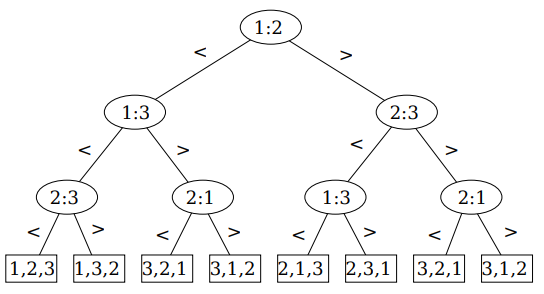
\includegraphics[scale=0.7]{selection}
\end{center}
An correct sorting algorithm must be able to produce each permutation of input (or: must sort any permutation of e.g. $\{1,...,n\}$)\\
A necessary condition is that each of the n! permutations must appear as leaf of decision tree\\
\textbf{Lower bound for worst case}\\
Length of longest path from root of decision tree to any leaf (height) represents worst case number of comparisons for given value of n.\\
For given n, lower bound on heights of all decision trees where each permutation appears as leaf is thus lower bound on running time of \textbf{any comparison based sorting algorithm}\\
\subsubsection{Theorem}
Any comparison based sorting algorithm requires $\Omega (n\log n)$
\subsubsection{Proof}
\begin{itemize}
\item Sufficient to determine minimum height of a decision tree in which each permutation appears as a leaf
\item Consider decision tree of height h with $\ell$ leaves corresponding to a comparison sort on n elements
\item Each of the n! permutations of the input appears as some leaf: $\ell\geqslant n!$
\item Binary tree of height h has at most $2^h$ leaves: $\ell\leqslant 2^h$
\item Together $n!\leqslant\ell\leqslant 2^h$ and therefore $2^h\geqslant n!$
\item Take logs: $h\geqslant \log (n!)=\Omega(n\log n)$
\end{itemize}
\subsection{Selection and adversaries}
\subsubsection{Lower bound via adversaries}
Adversary:
\begin{itemize}
\item Is second algorithm intercepting access to input
\item Gives answers so that there's always a consistent input
\item Tries to make original algorithm delay a decision by dynamically constructing a bad input for it
\item doesn't know what original algorithm will do in the future, must work for \textbf{any original algorithm}
\end{itemize}
To get a good lower bound, design a good adversary
\subsubsection{Finding max}
Goal: find max element in unsorted array\\
In an array of size n, can do this with n-1 comparisons\\
Same set-up as before: only comparisons are relevant
\paragraph{Theorem}
$ $\\
Any comparison based algorithm for this problem requires at least n-1 comparisons in the worst case
\paragraph{Proof}
$ $\\
After $\leqslant n-2$ comparisons, $\geqslant 2$ elements never lost (a comp)
\begin{itemize}
\item Adversary can make any of them max and be consistent
\item Not enough info for algorithm to make a decision
\end{itemize}
Hence algorithm needs to make at least n-1 comparisons
\subsubsection{Representing Adversary's strategy}
\begin{enumerate}
	\item As a digraph:
	\begin{itemize}
	\item the elements of array are the nodes
	\item if i loses to j, draw edge $i\rightarrow j$
	\item The adversary is consistent, so there cannot be any cycles, as that would lead to a contradiction
	\item The algorithm can stop when there is an element which can be reached from any other element following the path of directed edges, then you know the element is maximum. The smallest number of edges to make the graph connected is n-1
	\end{itemize}
	\item As a status update table with bits of info revealed:\\
	Each index i has status NL (never lost) or L (lost)\\
	When comparing i and j:
	\begin{center}
	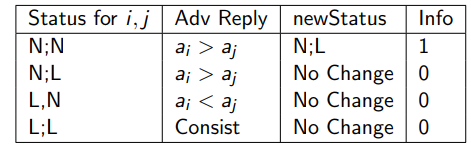
\includegraphics[scale=0.7]{adversary}
	\end{center}
	
\end{enumerate}
All the elements but one must lose at least once
\subsubsection{Finding 2nd largest}
Goal: find the 2nd largest element in an unsorted array
\paragraph{Theorem}$ $\\
Any comparison based algorithm for this problem requires at least $n+\lceil \log_2 n\rceil -2$ comparisons in the worst case
\paragraph{Observations}
\begin{enumerate}
	\item Any correct algorithm must also determine the max. $n-1$ elements most lose $\geqslant 1$ comparisons
	\item The 2nd largest must lose to max directly (there is no other element that it could lose to)
	\item If max had direct comparisons with m elements, then m-1 of these elements must lose $\geqslant 2$ comparisons
	\item Hence, at least $n-1+m-1=n+m-2$ comparisons are required
\end{enumerate}
\subsubsection{Adversary's strategy}
\paragraph{Lemma}
Adversary can force $\lceil\log_2 n\rceil$ comparisons involving max
\paragraph{Proof}$ $\\
Adversary assigns weight $w_i$ to each input element $a_i$\\
Initially all $w_i=1$, then update using these rules
\begin{center}
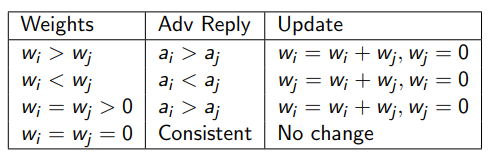
\includegraphics[scale=0.7]{strategy}
\end{center}
If the weights are equal and positive then the adversary makes a random decision
\subsubsection{Analysis}
\begin{itemize}
\item $w_i=0$ $\Leftrightarrow$ i lost $\geqslant 1$ comparison
\item Weight of an element at most doubles after a comparison (because you are shifting the smaller weight to the larger one)
\item If max is involved in m comparisons, its weight is $\leqslant 2^m$
\item In the end, max accumulates all the weight, so $n\leqslant 2^m$ (all elements feeding into max)
\item Taking logs, $\log_2 n\leqslant m$, as required
\end{itemize}
To conclude, Adversary can force $n+\lceil \log_2 n \rceil -2$ comparisons
\subsubsection{Finding 2nd largest: Algorithm}
Here's an algorithm that matches out lower bound.\\
Consider a knock out tournament: players= array elements\\
Think a balanced tree, leaves-array elements. With array of size n, the height of the tree is $\lceil \log_2 n\rceil$\\
Play the tournament to find max: this takes n-1 comparisons.\\
Consider the $\lceil \log_2 n\rceil$ elements who lost directly to max.\\
2nd largest overall=largest among those.\\
Find it with $\lceil \log_2 n\rceil-1$ comparisons.\\
Altogether, this used $n+\lceil\log_2 n\rceil -2$ comparisons
\subsubsection{Finding kth largest}
Let $C_k$ be the number of comparisons necessary and sufficient to find the kth largest element in an array of size n\\
The exact value of $C_k$ is known for
$$k=1,2,n-1,n$$
For the other values of k, this is open.\\
Though there are known bounds on $C_k$
\end{document}